% !TEX root = ../DP_Vik_Tomas_2013.tex
% pokyny
% Z uživatelského hlediska je velmi výhodné před nákupem zboží prozkoumat trh pomocí internetových srovnávačů. Zatím ovšem není snadno dostupná služba, která by uživateli umožnila vytvořit si hypotetický seznam zboží, které zvažuje koupit.

% *Vytvořte rešerši stávajících systémů zabývajících se organizací nákupních seznamů.
% *Zjistěte možnosti a strategii napojení na systémy zabývající se srovnáním a sledováním cen.
% *V souladu s touto rešerší poté analyzujte, navrhněte a implementujte webovou aplikaci, která bude umožňovat přidávat, sledovat, prioritizovat a kategorizovat zboží, zobrazovat jeho cenu a její vývoj.
% *Webovou aplikaci implementujte v jazyce Ruby ve vhodném frameworku.
% *Pro prioritizaci navrhněte a implementujte vhodné algoritmy.
% *API webové aplikace bude navrženo s ohledem na budoucí integraci s dalšími systémy (např. srovnávače cen apod.).
%
% - optimalizace na mobilni prohlizece, autocomplete nefunguje, drag'n drop
% - kompatibilita s prohlizecema

% - vyvoj@jagu.biz - Michal Přibyl - Oponent - zkontaktovat
\chapter{Rešerše}
První kapitola je věnovaná popisu problematiky této práce a přehledu aplikací, ktere řeší stejné nebo podobné problémy.
Nejdříve se zabývá přímými konkurenty výsledné aplikace. Zde je shrnuta funkcionalita webových aplikací, které umožňují organizaci nákupních seznamů.
Dále se zabývá aplikacemi, které mají nějakou významnou funkčnost vhodnou pro výslednou aplikaci. Jedná se o aplikace, které se nějakou svojí částí specializují na organizaci informací. Konec kapitoly je věnován technologickému aspektu práce. Budou shrnuty technologie, na kterých je v dnešní době možné postavit webové aplikace.
Na konci každé podkapitoly budou shrnuty slabé a silné stránky jednotlivých technologií.

\section{Nákupní seznamy}
\label{sec:nakupni-seznamy}
V následujících sekcích je popsána funkčnost hotových aplikací zabývajících se organizací nákupního seznamu. Všechny zmíněné aplikace jsou již v produkci a jsou zaštítěny velkými internetovými společnostmi.

\subsection{Google ShoppingList}
Webová aplikace doplňující službu Google Nákupy. Podporuje jednoduché přidání zboží. U přidaných položek zobrazuje následující informace a umožňuje podle těchto informací i řadit položky na seznamu:
\begin{itemize}
\item \textbf{Datum přidání položky}
\item \textbf{Nejnižší aktuální cena} - Služba Google Nákupy má informace o ceně získané z většího množství obchodů. U věci na seznamu zobrazuje nejnižší možnou cenu. Jiná než tato cena nelze zobrazit.
\item \textbf{Hodnocení produktu}
\end{itemize}
Zboží přidané do seznamu se dělí do dvou kategorií resp. seznamů. První seznam se nazývá Shopping List a jedná se o privátní nákupní seznam. Položky v tomto seznamu se zobrazují pouze uživateli, kterému seznam patří. Druhý seznam se nazývá seznam přání a je možné na něj zkopírovat odkaz. Tento odkaz následně uživatel odešle komukoli, s kým chce svůj seznam přání sdílet. Položky lze přesouvat mezi seznamy tlačítkem \emph{Sdílet}/\emph{Zrušit sdílení}.
Zboží v seznamu přání je primárně určeno pro ostatní uživatele, aby jej mohli koupit uživateli, který seznam přání vytvořil. Například jako vánoční, narozeninový, nebo svatební seznam přání. Seznam přání je vidět na obrázku \ref{fig:google-shoppinglist}

Další funkčnost, kterou nabízí tento seznam je:
\begin{itemize}
\item Přidání poznámky k položce - uživateli je umožněno přidat poznámku k položce na seznamu.  Tato poznámka je následně zobrazena u položky v hlavním přehledu.
\item Odebrání položky ze seznamu
\item Sdílení/Zrušení sdílení - viz. předchozí odstavec
\end{itemize}

\begin{figure}[htb]
\begin{center}
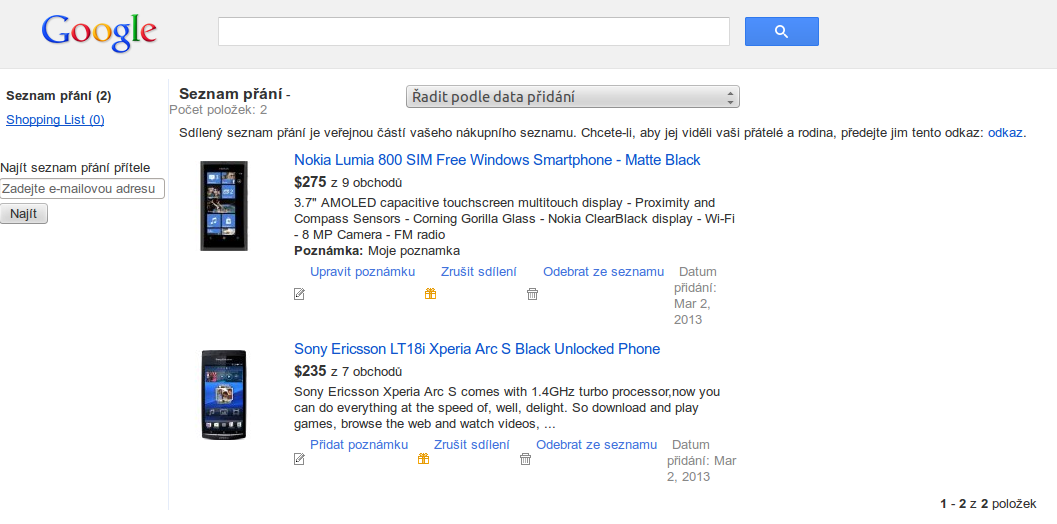
\includegraphics[width=120mm]{./pictures/google-shopping-list.png}
\caption{Google ShoppingList - základní obrazovka}
\label{fig:google-shoppinglist}
\end{center}
\end{figure}

\subsection{Amazon Wish List}
Amazon Wish List je funkcionalita poskytovaná komplementárně k internetovému obchodu Amazon.com. Služba umožňuje vytvářet a sdílet seznamy přání. Pro využívání této služby musí být uživatel přihlášen. Pokud se nepřihlášený uživatel pokusí přidat nějaký předmět do seznamu přání, je přesměrován na stránku přihlášení.

\subsubsection{Druhy přání}
Tato sekce se zabývá druhy přání ve službě Amazon Wish List. Přáním se v této službě rozumí tři věci:
\begin{itemize}
\item Produkt z internetového obchodu Amazon.com
\item Internetová stránka mimo Amazon.com
\item Nápad na přání (tzv. idea)
\end{itemize}

\paragraph{Produkt internetového obchodu Amazon.com}
\label{par:produkt-amazon}
Toto přání reprezentuje jedna k jedné produkt v internetovém obchodu Amazon.com. Toto přání vznikne tak, že přihlášený uživatel klikne na stránce produktu v obchodě Amazon.com na tlačítko \emph{Add To Wish List}. U takovéhoto přání se ukazuje minimální možná cena, popis i obrázek. Tedy maximální množství informací, které je aplikace schopna k přání uchovat.

\paragraph{Internetová stránka mimo Amazon.com}
Toto přání reprezentuje jakoukoliv internetovou stránku. Takovéto přání vznikne jedině pomocí pluginu Amazon Wish List Button. O této funkcionalitě pojednává samostatná podkapitola \ref{sec:amazon-wishlist-button}.

\paragraph{Nápad na přání}
Nápad na přání je funkcionalita, která umožní uživateli zadat nápad na přání pouze jako text (název přání). Tento nápad se uloží mezi ostatní přání. Místo obrázku přání je ovšem zobrazen obrázek nalepovacího štítku a na něm je napsáno "I Want". Nápad na přání je vidět na obrázku \ref{fig:amazon-wishlist-idea}. Každý nápad na přání má u sebe tlačítko \emph{Top search results} které najde pro popis nápadu produkty z obchodu Amazon.com. Takto nalezené produkty je možné okamžitě přidávat do seznamu. Nápad na přání přitom v seznamu zůstává, dokud jej uživatel neodstraní.

\begin{figure}[htb]
\begin{center}

\includegraphics[width=100mm]{./pictures/amazon-wishlist-idea.png}
\caption{Nápad na přání v Amazon Wish List}
\label{fig:amazon-wishlist-idea}
\end{center}
\end{figure}

\subsubsection{Amazon Wish List Button}
\label{sec:amazon-wishlist-button}
Amazon Wish List poskytuje plugin\footnote{Také zásuvný modul - software, který nepracuje samostatně, ale jako doplňkový modul jiné aplikace a rozšiřuje její funkčnost.} do všech majoritních internetových prohlížečů\cite{website:amazon:plugin}. Po nainstalování pluginu do prohlížeče si může uživatel přidat tlačítko \emph{Amazon Wish List Button} do ovládacího panelu prohlížeče. Po stisku tohoto tlačítka se otevře dialog. (Obrázek \ref{fig:amazon-wishlist-plugin})

\begin{figure}[htb]
\begin{center}
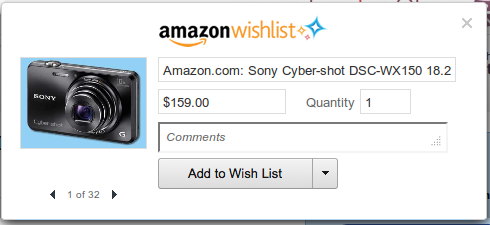
\includegraphics[width=100mm]{./pictures/amazon-wishlist-plugin.png}
\caption{Dialog zobrazený po stisku Amazon Wish List Button}
\label{fig:amazon-wishlist-plugin}
\end{center}
\end{figure}

Přidat je možné buď produkt z obchodu Amazon.com. V tomto případě se načtou všechna data, která se u přání ukladájí, a není rozdíl v použití pluginu oproti stisknutí tlačítka "Add to Wish List" na stránce produktu (viz. kapitola \ref{par:produkt-amazon}).

Dále plugin podporuje funkci přidání přání v podobě jakékoli stránky. Tedy je možné přidat do Amazon Wish List například zboží z českého internetového obchodu. Jako obrázek k přání si uživatel může zvolit libovolný obrázek ze stránky. Jako název přání se použije titulek stránky\footnote{Obsah HTML tagu <title> ve zdrojovém kódu stránky}, popisek se k přání žádný nepřidává. Uživatel si ještě k přání muže doplnit cenu před tím než ho uloží do seznamu.

\subsection{WishList.com}
WishList.com je webová aplikace zaměřená primárně na vytváření seznamu přání. U každého seznamu podporuje sdílení a také podporuje nastavení události k seznamu a data této události. Většina seznamů má tyto hodnoty vyplněny a jsou to například seznamy přání k narozeninám, vánocům nebo seznam svatebních darů. Jako zdroj dat používá internetový srovnávač PriceGrabber.com, který je popsán v rešerši srovnávačů.

WishList.com neumožňuje přihlášení pomocí OpenID. Uživatel se může přihlásit pomocí svého Facebook účtu, nebo zaregistrovat klasickou metodou, kdy zadá svůj email, přihlašovací jméno a heslo.

Uživatel může vytvářet nové seznamy přání a nová přání. Při vytvoření nového seznamu zadává uživatel jeho název, obrázek, omezení přístupu (veřejný, pouze přátelé, soukromý), popis, osobní poznámky, osobu, která si věci přeje, název a datum události. Pouze název seznamu je povinné pole. Seznam je navíc možné zabezpečit heslem.

Při přidávání přání je možné zadat prodejce předmětu, název předmětu, popis předmětu, cenu, množství, prioritu, poznámky k přání, seznam přání do kterého bude přání přidáno, příjemce přání a poté URL produktu a URL obrázku produktu. Povinným polem je pouze název předmětu.

Vytvořený seznam je možné sdílet pomocí URL. Pokud si seznam prohlíží jiný uživatel než ten, který jej vytvořil, může si tento uživatel zarezervovat přání, což znamená že koupí předmět a dá jej uživateli, který si jej přál.

Seznam přání i jednotlivá přání je možné sdílet s ostatními uživateli pomocí tlačitka \emph{Share this WishList} resp. \emph{Share this Wish}. Sdílení je možné pomocí služeb Facebook, Myspace, Google, Twitter, Email a dalších více než 300 sociálních služeb. Na sdílení je pravděpodobně použit nějaký plugin.

Aplikace WishList podporuje vyhledávání zboží pomocí více zmíněného PriceGrabber.com. Pokud má zboží pouze jednoho prodejce, přesměruje uživatele tlačítko \emph{Buy} u přání přímo na stránku prodejce. Jinak je uživatel přesměrován na stránku s výběrem prodejců. Tato stránka se nachází stále na WishList.

Po přidání přání, které bylo nalezeno vyhledáváním, je uživateli zobrazena zpráva, která se ptá, jestli chce uživatel opravdu čekat a nekoupí si své přání rovnou. Tato výzva je vidět na obrázku \ref{fig:wishlist-buynow}.

\begin{figure}[htb]
\begin{center}
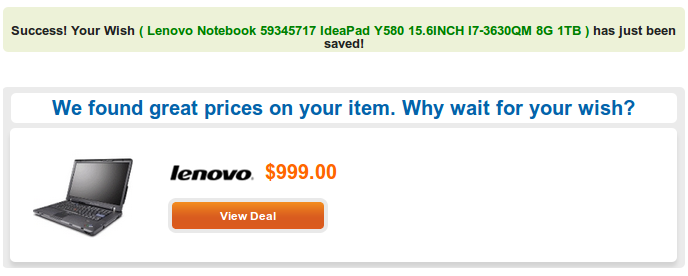
\includegraphics[width=100mm]{./pictures/wishlist-buynow.png}
\caption{Výzva k okamžitému zakoupení přání}
\label{fig:wishlist-buynow}
\end{center}
\end{figure}

Přehled přání je vidět na obrázku \ref{fig:wishlist-wishlist}.

\begin{figure}[htb]
\begin{center}
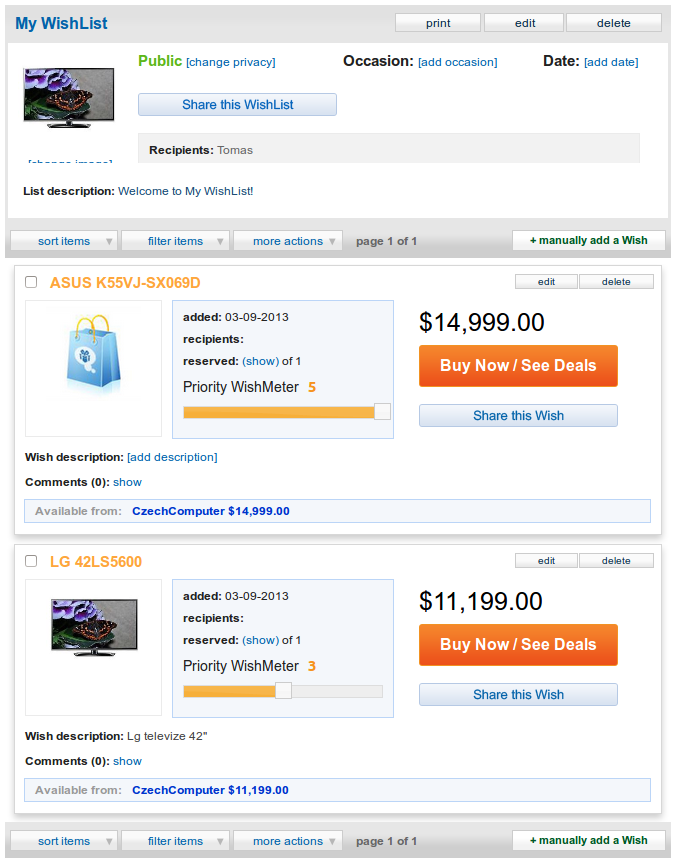
\includegraphics[width=100mm]{./pictures/wishlist-wishlist.png}
\caption{Hlavní přehled přání na stránce WishList.com}
\label{fig:wishlist-wishlist}
\end{center}
\end{figure}

\subsubsection{Nedostatky WishList.com}
Cena u přání jde zadat pouze v dolarech. WishList umožňuje vyhledat zboží pro přání, u kterých není uvedena URL produktu, ale vyhledávání nefunguje kompletně, nenašlo nic pro výraz "iphone", pro který PriceGrabber (zdroj dat pro WishList) nalezne několik stovek výsledků.

\section{Srovnávače cen}
\label{sec:srovnavace-cen}
Tato kapitola poskytuje rešerši aplikací známých jako srovnávače cen, jejichž cílem je poskytnout uživateli širší pohled na trh. Tyto aplikace umožňují u jednoho produktu srovnat cenu v několika internetových obchodech. V rešerši jsou zpracovány jako potencionální zdroje dat pro výslednou webovou aplikaci.

\subsection{Standardní funkce všech srovnávačů}
V této sekci jsou popsány tři základní funkce, které podporují všechny zmíněné srovnávače cen. Lze říci, že se jedná o funkce, které definují srovnávač cen jako takový.

\subsubsection{Vyhledávání}
Každý ze zmíněných vyhledávačů podporuje fultextové vyhledávání zboží\footnote{(Z ang. full – celý, plný a text) speciální způsob vyhledávání informací v databázích nebo v textových souborech, které jsou obvykle předem připraveny, tj. indexovány, aby bylo možno nalézt libovolné slovo (řetězec znaků) v nejkratším možném čase.}. Toto vyhledávání probíhá nad databází veškerých výrobků, které aplikace (srovnávač) obsahuje. Vyhledávány jsou jednotlivé výrobky, u nichž jsou agregovány ceny z jednotlivých obchodů, tzn. výrobek se zobrazí v ideálním případě\footnote{Produkt může mít v různých obdhodech různá jména, takové produkty se ne vždy podaří srovnávači agregovat.} pouze jednou, přestože srovnávač má informace o několika obchodech, které jej poskytují.

Dále umožňují srovnávače vyhledávání po kategoriích. Na domovské stránce srovnávače je uživateli nabídnut seznam kategorií a významných podkategorií. Uživatel po rozkliknutí kategorie vidí vybrané zboží z dané kategorie a případně také podkategorie, pokud nějaké jsou.

Uživateli je také umožněno filtrovat zboží na základě jeho parametrů. Parametry podle kterých se filtruje je možné rozdělit na několik druhů:
\begin{itemize}
\item \textbf{Společné pro veškeré zboží} - například cena výrobku, nebo značka výrobce.
\item \textbf{Rozlišné pro každou kategorii} - parametry, které dávají smysl pouze v dané kategorii. Např. velikost ohniska u objektivů nemá smysl nikde jinde. Stejně tak velikost uhlopříčky nemá smysl v kategoriích, kde není žádné zobrazovací zařízení.
\end{itemize}

\paragraph{Databáze zboží}
Srovnávače cen plní svojí databázi zboží z dat od zákazníku. U porovnávaných srovnávačů je princip následující: Obchod, který chce, aby jeho zboží bylo vidět ve srovnávači, vystaví veřejně XML soubor, ve kterém je detailní popis každého produktu včetně informací jako způsob a doba doručení.\cite{website:heureka:registrace-obchodu}

\subsubsection{Srovnávání cen}
Každá aplikace podporuje srovnání cen u zboží. U většiny zboží v databázi je přiřazen větší počet obchodů. Díky shromáždění cen z jednotlivých obchodů je poté srovnávač schopný zobrazit u zboží nejnižší a nejvyšší cenu. U zboží je zároveň zobrazen přehled všech obchodů ve kterých je zboží nabízeno. Několik obchodů je zpravidla doporučeno srovnávačem. K tomu mohou mít obchody ještě seznam ocenění získaných srovnávačem.

Zpravidla je u obchodu zobrazena také dostupnost zboží, případně cena dopravy. Díky těmto informacím uživatel okamžitě vidí, kdy může zboží mít a kolik zaplatí navíc oproti ceně uvedené v obchodě.

Díky pravidelnému sledování cen zboží v obchodech má srovnávač chronologická data o ceně zboží. Díky této vlastnosti nabízí funkcionalitu graf historie cen. V grafu je zanesena cena zboží řádově za několik uplynulých měsíců. Tento graf pomáhá uživateli v rozhodnutí o koupi. Uživatel vidí, zdali se cena právě nachází pod nebo nad dlouhodobým průměrem.

\subsubsection{Uživatelská zpětná vazba}
Srovnávače zpravidla umožňují uživatelům hodnotit obchody, i zboží. U obchodů se hodnotí parametry jako dodací lhůta, přehlednost obchodu a kvalita komunikace. U zboží je výběr parametrů pro hodnocení jako při filtrování zboží podle atributů. V každé kategorii se hodnotí relevantní parametry zboží. 

Hodnocení většinou probíhá na principu jedné až pěti hvězdiček, případně shrnutí kladů a záporů.

Hodnocení produktu na srovnávači Heureka.cz je vidět na obrázku \ref{fig:heureka-hodnoceni-produktu}

\begin{figure}[htb]
\begin{center}
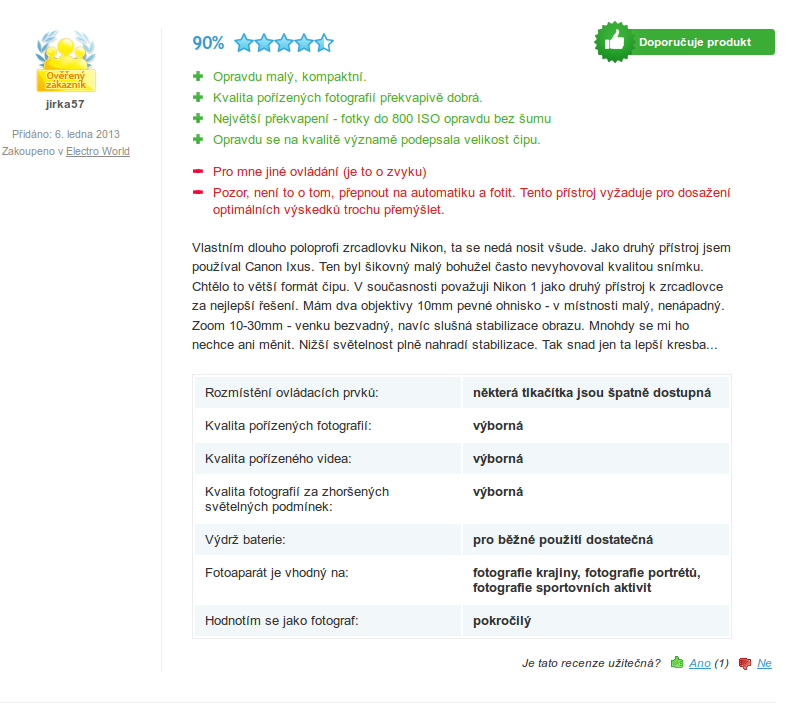
\includegraphics[width=100mm]{./pictures/heureka-hodnoceni-produktu.png}
\caption{Hodnocení produktu Nikon 1 J1 na srovnávači Heureka.cz}
\label{fig:heureka-hodnoceni-produktu}
\end{center}
\end{figure}

\subsection{Heureka.cz}
Interaktivní nákupní rádce Heureka.cz byl založen společností Miton v roce 2007, kdy ihned zaujmul zajímavým nápadem zkombinování mnoha užitečných možností do jednoho celku. Následně rozšiřuje svou působnost i na Slovensko a zakládá slovenskou verzi Heureka.sk (založena v r. 2008). \cite{website:wiki:heureka}

\subsubsection{Přidaná funkcionalita}
Další důležitou funkčností je hlídač ceny. Přihlášenému uživateli je umožněno na zboží nastavit hlídače ceny a poté co cena v nejlevnějším obchodě klesne pod zadanou částku, uživatel dostane email s upozorněním.

\begin{itemize}
\item \textbf{Záruka vrácení peněz u některých obchodů} - U smluvních partnerů je Heureka.cz schopná se zaručit za bezproblémový nákup. Pokud by zákazník zaplatil za zboží a to mu nebylo dodáno, Heureka.cz mu vrátí peníze.
\item Varování před obchody, které nedodržují své obchodní podmínky
\item Sledovaní slev a novinek na trhu
\end{itemize}

\subsection{Zboží.cz}
Zboží.cz je srovnávač cen vytvořený společností Seznam.cz. Na Zboží.cz je registrováno více než 16000 obchodů a více než 62 milionu produktů. Denně navštíví srovnávač 180000 uživatelů a každý uživatel v průměru na stránce stráví 39 min.\cite{website:zbozi-about}
Zboží.cz je satelitní web společnosti Seznam.cz.
\footnote{Satelitní web je rozšířená a propracovanější forma tzv. microsite (jinak také minisite či weblet), jde o speciální samostatný web plnící funkce, které se na hlavní webovou prezentaci nehodí, nebo s ní dokonce nesouvisejí.}
\subsubsection{Přidaná funkcionalita}
Zajímavou funkcionalitou je srovnávání zboží. Uživatel má možnost přidat produkt do srovnání zboží pomocí tlačítka \emph{Přidat do porovnání} viz obrázek \ref{fig:zbozicz-srovnat}. Tím se zboží přidá do seznamu. Tento seznam obsahuje pro každý produkt jeden sloupec a v každém řádku je nějaká vlastnost produktu. Pokud produkt ve srovnání nemá danou vlastnost, je v dané buňce nápis \emph{Neznámý}.

\begin{figure}[htb]
\begin{center}

\includegraphics[width=40mm]{./pictures/zbozicz-srovnat.png}
\caption{Tlačítko pro srovnání zboží}
\label{fig:zbozicz-srovnat}
\end{center}
\end{figure}

Výsledek takového srovnání je poté vidět na obrázku \ref{fig:zbozicz-srovnani}.

\begin{figure}[htb]
\begin{center}
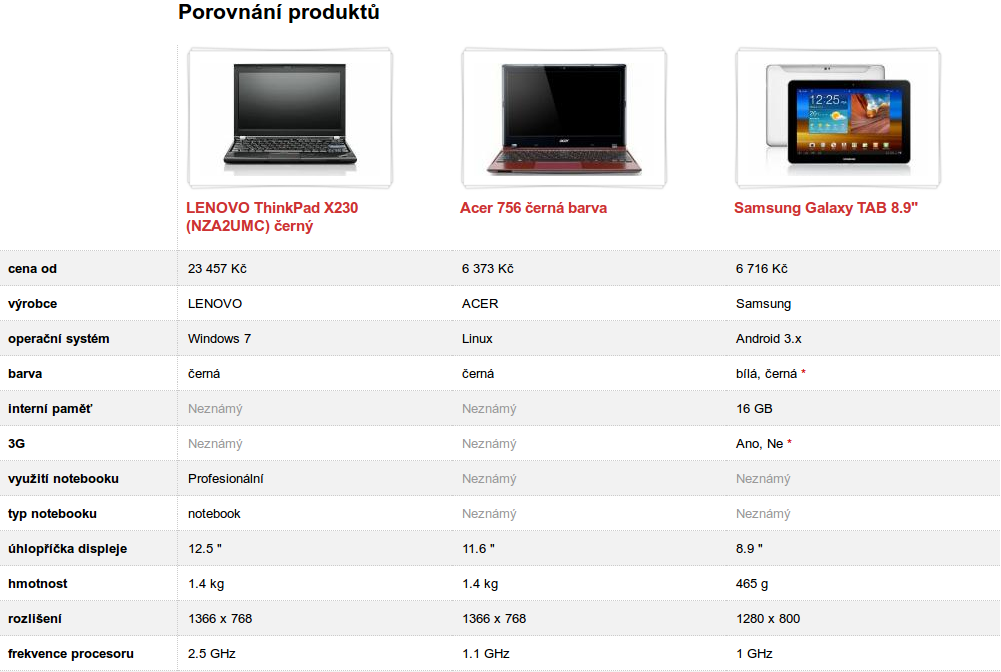
\includegraphics[width=130mm]{./pictures/zbozicz-srovnani.png}
\caption{Výsledek srovnání zboží na serveru Zboží.cz}
\label{fig:zbozicz-srovnani}
\end{center}
\end{figure}

\subsection{PriceGrabber}
PriceGrabber je služba pro srovnávání cen. Jejími partnery je více než 13000 prodejců. Poskytuje volně informace o milionech produktů ve více než 25 kategoriích. Společnost také slouží jako datový zdroj pro další prodejní služby jako AOL Shopping, Bing Shopping aj. \cite{website:wiki:pricegrabber}

PriceGrabber byl první srovnávač, který zahrnul informace o daních a poplatcích za přepravu do srovnávání. \cite{website:wiki:pricegrabber}

\subsubsection{Přidaná funkcionalita}
PriceGraber obsahuje funkčnost v Čechách poprvé zavedenou portálem Slevomat.cz\footnote{Slevomat je český server hromadného nakupování založený Tomášem Čuprem, Petrem Bartošem a Romanou Sudovou.}. Tato funkčnost se nazývá ``Local Deals'' a umožňuje uživateli pořizovat zvýhodněné služby a/nebo zboží.

PriceGrabber obsahuje velké množství tzv. ``Buying Guiedes'', tedy příručky k nákupu, které poskytují základní rady a doporučení pro koupi daného typu zboží. Obsahuje tedy například příručku pro nákup klimatizace.

\section{Aplikace s žádanou funkčností}
\label{sec:aplikace-s-zadanou-funkcnosti}
Tato kapitola popisuje několik aplikací, které svým zaměřením nesplňují přímo podmínky této práce, ale část jejich funkcionality by byla pro výslednou aplikaci přínosem.

\subsection{Astrid}
\label{sec:astrid}
Astrid je aplikace pro správu úkolů. Mezi její klíčové funkce patří vytváření, úprava a kategorizace úkolů. Tato aplikace byla původně navržena pro mobilní zařízení a operační systém Android, nyní má aplikace také webové rozhraní, jehož funkcionalita je předmětem této kapitoly.

Základní obrazovku aplikace je možné vidět na obrázku \ref{fig:astrid}

\begin{figure}[htb]
\begin{center}
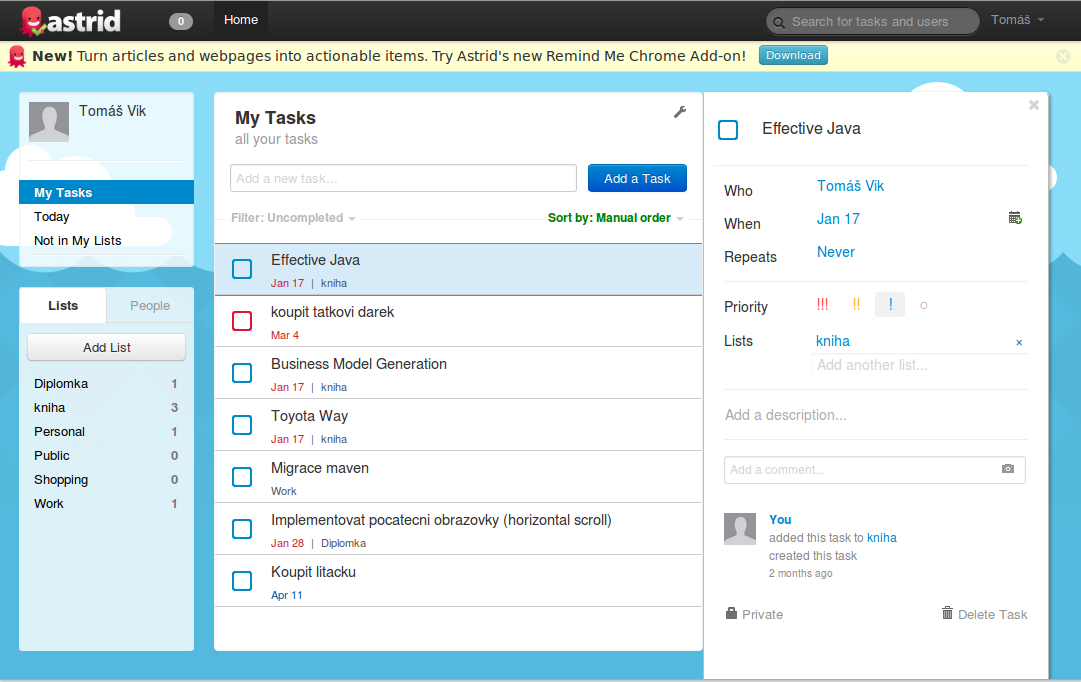
\includegraphics[width=130mm]{./pictures/astrid.png}
\caption{Základní strana webové aplikace Astrid.com}
\label{fig:astrid}
\end{center}
\end{figure}

Na základní straně je vidět jednoduchost aplikace. Přidání úkolu proběhne pomocí vyplnění názvu úkolu a stisknutí tlačítka \emph{Add a Task}. Tím se úkol zobrazí v seznamu ostatních úkolů a jeho detaily už je pak možné nastavit stejně jako u všech ostatních úkolů.

Editace úkolu se provede kliknutím na daný úkol v seznamu. V pravé části obrazovky se zobrazí panel s detailními informacemi o úkolu.

Hlavní seznam úkolů je možné řadit pomocí několika kritérií. Mimo standardní kritéria jako priorita a datum přidání je možné řadit také manuálně (tzv. \emph{Manual order}). Uživatel může kliknout na položku na seznamu a přetáhnout ji mezi jakékoli 2 jiné položky, nebo na začátek/konec seznamu. Takto je uživateli umožněno seřadit si úkoly dle libosti.

Každý úkol náleží do 0-n seznamů. Tyto seznamy je možné libovolně vytvářet a mazat. Přidáváním přání do seznamů je uživateli umožněna další úroveň kategorizace. U každého seznamu se ukazuje panel s informacemi o aktuálních aktivitách v seznamu (např. vytvoření, dokončení a úprava úkolu).

Mazání přání probíhá pomocí tlačítka \emph{Delete Task} v panelu s informacemi o úkolu. Tímto tlačítkem se úkol okamžitě smaže, ale uživateli se zobrazí upozornění v horní části obrazovky. V tomto upozornění je také tlačítko na vrácení smazání přání viz. obrázek \ref{fig:astrid-undo}. Toto upozornění po několika málo vteřinách zmizí. Poté může uživatel obnovit přání ze seznamu akcí provedených nad seznamem přání.

\begin{figure}[htb]
\begin{center}

\includegraphics[width=130mm]{./pictures/astrid-undo.png}
\caption{Panel informující o smazání úkolu umožňuje vrátit operaci zpět}
\label{fig:astrid-undo}
\end{center}
\end{figure}


Tento způsob mazání je lepší než klasický dialog pro potvrzení smazání, pokud jsou mazané položky relativně nedůležité pro uživatele a manipuluje s nimi ve velkém (což je případ právě úkolů). Uživatel má v naprosté většině případů úmysl úkol smazat, ale pokud to udělá omylem, může smazání bezpečně vrátit. 

V základním rozložení stránky je komponenta (na obrázku \ref{fig:astrid-tasklist}), která umožňuje přecházet mezi seznamy úkolů, případně procházet osoby, se kterými mám aplikaci propojenou. Tato komponenta je přítomna na každé stránce aplikace a uživatel tedy kdykoli může přejít na nějaký konkrétní seznam svých úkolů.

\begin{figure}[htb]
\begin{center}
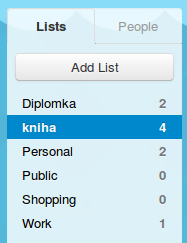
\includegraphics[width=40mm]{./pictures/astrid-tasklist.png}
\caption{Komponenta ze které je možné kdykoli přejít na konkrétní seznam úkolů.}
\label{fig:astrid-tasklist}
\end{center}
\end{figure}

Aplikace umožňuje také poslat uživateli email s upozorněním na blížící se termín splnění přání.

Poslední zajímavá funkčnost je \emph{Remind Me button}, tedy tlačítko, které si může jakýkoli uživatel umístit na webové stránky a pokud na něj klikne návštěvník této stránky, je mu automaticky přidán úkol do seznamu úkolů. HTML kód tlačítka se vytvoří pomocí jednoduchého formuláře, do kterého se zadá nadpis úkolu, za jak dlouho (popř. kdy) má být úkol splněn, název internetové stránky, na které je tlačítko umístěno a URL které se úkolu týká.

Technicky je celá aplikace řešena pomocí AJAX. To znamená, že se stránka nenačítá znovu po každém kliknutí na tlačítko/odkaz, ale pouze se doplňují data do potřebných částí stránky. K určení cesty na stránce se používá tzv. identifikátor fragmentu\footnote{Krátký řetězec znaků označující zdroj, který je podřízený jinému, primárnímu, zdroji. Primární zdroj je určen URI, identifikátor fragmentu je od URI oddělen znakem \#.}. Frontend aplikace je postaven na technologii twitter bootstrap.
%https://twitter.com/astrid/status/222836247498985472

\section{Technologie pro vývoj aplikace}
Tato část rešerše se zabývá technologiemi, ve kterých je možné implementovat webovou aplikaci. V každé podkapitole je nejprve popsán programovací jazyk a k němu následují nejpoužívanější frameworky pro implementaci webových aplikací.
\subsection{Java}
Java je objektově orientovaný programovací jazyk, který vyvinula firma Sun Microsystems a představila 23. května 1995.

Java je jedním z nejpoužívanějších programovacích jazyků na světě. Podle Tiobe indexu je Java nejpopulárnější programovací jazyk.[1] Díky své přenositelnosti je používán pro programy, které mají pracovat na různých systémech počínaje čipovými kartami (platforma JavaCard), přes mobilní telefony a různá zabudovaná zařízení (platforma Java ME), aplikace pro desktopové počítače (platforma Java SE) až po rozsáhlé distribuované systémy pracující na řadě spolupracujících počítačů rozprostřené po celém světě (platforma Java EE). Tyto technologie se jako celek nazývají platforma Java. Dne 8. května 2007 Sun uvolnil zdrojové kódy Javy (cca 2,5 miliónů řádků kódu) a Java bude dále vyvíjena jako open source.
\subsubsection{Spring MVC}
Spring MVC Web framework funguje na principu návrhového vzoru MVC. Ten znamená jasné oddělení perzistence, byznys logiky a prezentační vrstvy. Napříč těmito vrstvami je doménový model, tedy Java třídy reprezentující datový model aplikace\cite{liu2006research}.

\begin{figure}[htb]
\begin{center}
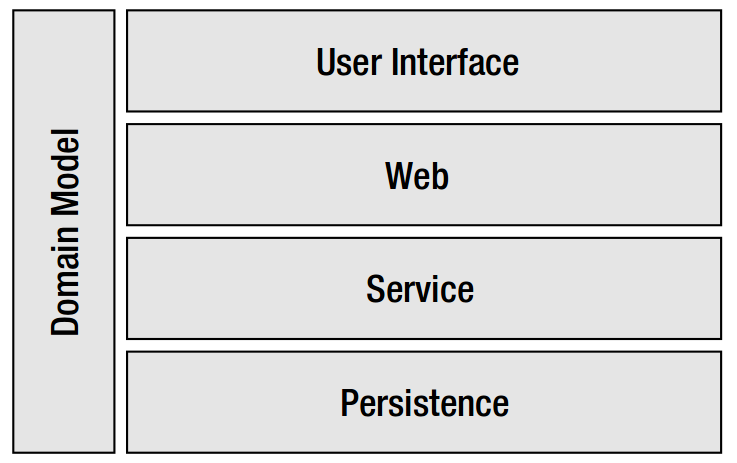
\includegraphics[width=50mm]{./pictures/spring-mvc-layers.png}
\caption{Aplikační vrstvy Spring MVC aplikace \cite{liu2006research}}
\label{fig:spring-mvc-layers}
\end{center}
\end{figure}

Jak název napovídá Spring MVC framework je postaven na aplikačním frameworku Spring. Využívá jeho základní mechanismy, jako Inversion Of Control kontejner a Dependency Injeciton.

Výhodou Spring MVC je, že je možné vybrat různé knihovny pro řešení specifických problémů aplikace. Např. knihovnu pro řešení prezistence (MyBatis, Hybernate), nebo knihovnu pro view (JSP, Velocity, FreeMarker, atd.)\cite{liu2006research}.

\subsection{Ruby}
\label{sec:ruby}
Ruby je dynamický, reflexivní, objektově orientovaný programovací jazyk, který kombinuje syntaxi inspirovanou jazykem Perl s funkcemi podobnými Smalltalku. Ruby je také ovlivněný jazyky Eiffel a Lisp. Ruby byl prvotně navržen a vyvinut v polovině devadesátých let minulého století japoncem Yukihiro "Matz" Matsumoto.

Ruby podporuje několik programovacích paradigmat. Mimo jiné funkcionální, objektově orientované, imperativní a reflektivní. Ruby má dynamické typování a automatickou správu paměti. Je tedy v mnohých aspektech podobný jazykům Smalltalk, Python, Perl, Lisp, Dylan, Pike a CLU.

Současná verze jazyka je 1.9.3.
\subsubsection{Ruby on Rails}
\label{sec:ror}
Ruby on Rails je framework pro vývoj webových aplikací napojených na databázi, používající návrhový vzor Model-view-controller. Vytvořil jej dánský programátor David Heinemeier Hansson při práci na projektu Basecamp\cite{website:wiki:ror}.

Vše v Rails je založeno na jazyce Ruby. Na jazyce Ruby je založen Ajax v šablonách (view), odpovědi v controllerech i architektura aplikace v modelech obalujících databázi. Ke spuštění aplikace je třeba jen databáze.

Mezi základní princip Rails patří Konvence má přednost před konfigurací, tedy programátor konfiguruje pouze ty části aplikace, které se liší od běžného nastavení. Vytvoří-li tedy např. model Person, aplikace bude data automaticky hledat v tabulce people. Chce-li, aby aplikace načítala data z tabulky staff, musí tak učinit výslovně.

Rails jsou postaveny na bázi návrhového vzoru Model-view-controller, který odděluje části aplikace zodpovědné za čtení a ukládání dat včetně manipulace s nimi (model), za zobrazení grafického rozhraní aplikace (view) a za část přijímající vstupy od uživatele a řídící zobrazení dat na výstupu (controller).

\subsubsection{Sinatra}
Sinatra je minimalistický framework\footnote{Zde se definice liší, například Alan Harris ve své publikaci Sinatra Up and Running uvádí, že sinatra není framework, ale podle autorova názoru definici tohoto slova naplňuje.} a doménově specifický jazyk\footnote{Doménově specifický jazyk je programovací jazyk, který je prostřednictvím vhodné abstrakce a výrazového slovníku zaměřen na omezenou, konkrétní problémovou doménu. V tomto případě jsou doménou Webové stránky.} založený na ruby. Neobsahuje žádné další knihovny, jako například ORM, nebo komplexní knihovny na práci s View. Je určen pro jednoduché webové aplikace, webové služby. Sinatra nevnucuje programátorovi žádný návrhový vzor, takže na rozdíl od velkého množství frameworků není postaven na MVC.\cite{harris2011sinatra}

Jak již bylo naznačeno v předchozím odstavci, Sinatra poskytuje minimální obal okolo HTTP dotazu a odpovědi. Celá knihovna je napsána v méně než 2000 řádcích\cite{harris2011sinatra}. Sinatra je vhodná pro drobnou aplikaci, kde je důležitá primárně jednoduchá syntaxe a přehlednost kódu. Není výjimkou, že celá webová aplikace postavená na Sinatře se nachází v jednom souboru\cite{harris2011sinatra}.

\subsection{Frontend frameworky}
Do této kategorie spadají veškeré aplikace/skripty/styly, které vývojáři usnadňují vývoj klientské části aplikace, tedy té části, kterou uživatel vidí ve svém prohlížeči. Tyto frameworky kombinují HTML a CSS návrhové prvky a k nim přidávají JavaScript funkcionalitu \cite{website:wiki:bootstrap}\cite{website:boilerplate}. Vývoj v těchto frameworcích spočívá v psaní klasického HTML, kterému vývojář přidává speciální třídy, které jsou nastylované frameworkem\cite{website:wiki:bootstrap}.

\subsubsection{Twitter Bootstrap}
Bootstrap byl vyvinut vývojáři Markem Ottem a Jacobem Thorntonem ve společnosti Twitter jako standard pro udržení konzistence napříč interními nástroji. Do té doby byly pro vývoj uživatelských rozhraní používány různé knihovny, což mělo za následek zvýšené náklady na údržbu.

V září 2011 byl framework uvolněn jako open-source. Nyní (duben 2013) je nejoblíbenějším projektem na Github.com s velice širokou komunitou vývojářů\cite{website:github-popular}.


Mezi mnohými funkcemi frameworku je například automatický 12-ti sloupcový mřížkový laout\footnote{Vývojář může jednotlivé komponenty vkládat do 12-ti sloupců kde každá komponenta může zabírat libovolný počet sloupců. Komponenty je možné vkládat do řádků.} a responzivní layout, který vhodně mění rozložení prvků v závislosti na velikosti okna prihlížeče\footnote{To je vhodné pro zobrazení jedné stránky na více typech zařízení (PC, tablet, mobilní telefon).}.

Na obrázku je vidět příklad jednoduché stránky přímo ze stránek frameworku. Zdrojový kód tvořící tuto stránku má 127 řádků kódu\cite{website:bootstrap-example}.

\begin{figure}[htb]
\begin{center}
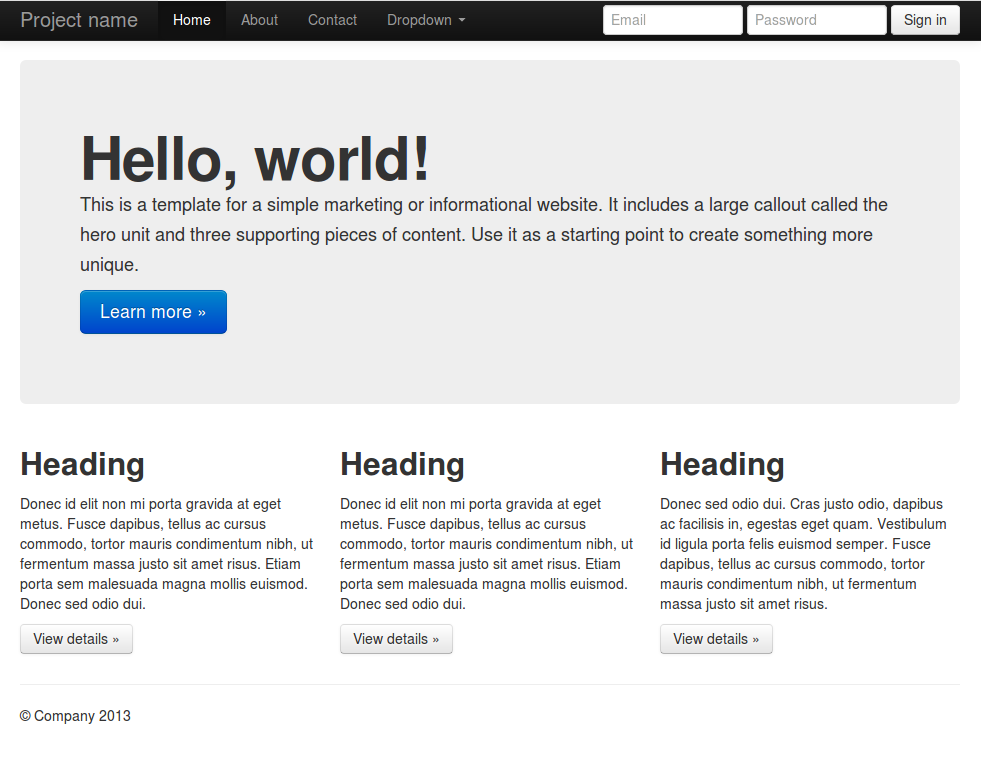
\includegraphics[width=80mm]{./pictures/bootstrap-example.png}
\caption{Příklad jednoduché stránky ve frameworku Twitter Bootstrap \cite{website:bootstrap-example}}
\label{fig:bootstrap-example}
\end{center}
\end{figure}

\subsubsection{HTML 5 Boilerplate}
V roce 2009 začal Paul Irish kopírovat často používané kusy svého HTML, CSS a JavaScript kódu do jednoho dokumentu. Tento dokument sestával pouze ze základních kusů kódu. Paul Irish od té doby začal vždy stavět nový projekt nad tímto dokumentem. Tím vzniknul frontend framwork HTML 5 Boilerplate, který byl poprvé uvolněn v lednu 2010 a pod svým nynějším názvem je od června 2010.\cite{website:boilerplate-history}

Tento projekt má za cíl obsahovat naprosté minimum, které potřebuje každý vývojář při své práci\cite{website:boilerplate-history}. Díky této myšlence, na které je framework postaven poskytuje spíše funkce, které lze využívat při tvorbě stránek než hotové komponenty, ze kterých by stránka šla přímo postavit.

\section{Možnosti napojení aplikace na systémy srovnávání cen}
Možnosti napojení aplikace na systémy srovnávání cen jsou v zásadě 2. Využití API samotného systému, nebo využití takzvaného web scrapingu viz. \ref{sec:webscraping}

\subsection{Napojení na API systému}
V tomto ohledu jsou možnosti vesměs omezené. Čeští poskytovatelé (Heureka.cz, Zboží.cz) API veřejně neposkytují a na svých stránkách neuvádí podmínky pro získání přístupu k jejich datům. Zahraniční poskytovatel PriceGrabber svoje API poskytoval formou webové služby. Toto API bylo veřejné a mohl je využívat kdokoli. Nyní je přístup k tomuto API znemožněn\cite{website:pricegrabber-api}. Například v rešerši zmiňovaný WishList je na tomto API postaven. Nyní je možné kontaktovat obchodní oddělení serveru a vyjednat s ním podmínky použití API.

Tato metoda má jasnou výhodu v několika aspektech. Nejdůležitějším aspektem je legalita. Pokud systém vystaví veřejně svoje API a uživatel dodrží podmínky jeho užití, nemůže dojít k porušení žádného zákona. Dalším důležitým aspektem je výkonnost. Komunikace přes webovou službu je jednoduchá, nezatěžuje zbytečně šířku pásma. Poskytovatel API přesně ví, jaké metody jsou volány za jakým účelem a může optimalizovat byznys logiku v implementaci webových služeb (cache, výkonnější DB atp.). Poslední důležitou výhodou je verzování API. U webových služeb je běžnou praxí tzv. verzování\cite{josuttis2007soa}. To znamená, že nová funkčnost webové služby nikdy neovlivní současnou verzi, namísto toho je nová funkčnost vystavena až v další verzi. Tím nemůže dojít k narušení funkčnosti klientské aplikace.

Nevýhodou API systému je v tomto konkrétním případě velmi omezený přístup a nutnost dohody s poskytovatelem ještě před testováním samotného API. Další nevýhodou je například jasně daný rozsah funkčnosti, který nemusí vždy korelovat s funkčností nabízenou například webovým rozhraním aplikace.

\subsection{Web Scraping}
\label{sec:webscraping}
Toto je metoda, která se používá k extrakci dat z datových stránek. Simuluje dotazy běžného uživatele a z nich získává data. Před nástupem webových služeb byla tato metoda hlavním způsobem, jak automatizovat získávání dat z webových stránek\cite{oreilly2007web}. Základní postup takovéto metody je následující:

\begin{enumerate}
\item Aplikace provede dotaz na předem danou URL. \newline \emph{Např. http://srovnavac.cz/produkt?id=1}
\item Aplikace dostane odpověď v podobě zdrojového kódu dotazované stránky.
\item Aplikace musí tomuto zdrojovému kódu porozumět, zpracovat ho a převést do interní reprezentace datové struktury.
\end{enumerate}

Web Scraping je tedy velmi přímočará metoda, jak získat jakákoli data, ke kterým má běžný uživatel přístup pomocí webového prohlížeče. Získávání dat tímto způsobem má opět několik výhod. První výhodou je jednoduchá implementace. Je třeba zjistit URL požadovaných zdrojů, umístění potřebných dat na stránce a ošetření případných chyb, které při získání dat mohou nastat. Další výhodou je transparentní dokumentace. Webové stránky jsou navrženy tak, aby je uživatel snadno pochopil, a tedy i programátor, který získává ze stránek data snadno pochopí co znamenají a kde se tato data nachází.

Web Scraping má na druhou stranu několik nevýhod. První nevýhodou jsou legální problémy spojené s tímto získáváním dat. V Čechách znám jediný případ kdy aplikace využívala tímto způsobem data cizího serveru. Jednalo se o aplikaci Pubtran, která využívala informace o jízdních řádech ze serveru \emph{jizdnirady.idnes.cz}. Autor aplikace František Hejl poté musel umístit do aplikace reklamní banery Idnes.

Další nevýhodou je závislost na konkrétním \emph{vzhledu}\footnote{V tomto kontextu se nejedná o vizuální podobu stránek, ale o podobu zdrojového kódu stránky.} webové aplikace. Pokud se rozhodne poskytovatel přepracovat svůj návrh stránek, poté je nutné této změně přizpůsobit také aplikaci, která ze stránek data získává.

Poslední nevýhodou je obtížně testování aplikace postavené na získávání dat touto metodou. Nikdy není zaručeno, že server nevrátí na dotaz nějakou stránku, se kterou aplikace nepočítá.

\section{Vyhodnocení rešerše}
V následujících bodech bude zhodnocena veškerá funkcionalita pospaná v kapitolách \ref{sec:nakupni-seznamy} a \ref{sec:srovnavace-cen}. Půjde především o zhodnocení silných a slabých stránek zmiňovaných systémů a aplikací. 

%a \ref{sec:aplikace-s-zadanou-funkcnosti}

\subsection{Přímí konkurenti výsledné aplikace}
Výhodou řešení od firem Amazon a Google je skutečnost, že jsou to projekty velkých, na internetu prosazených, společností. Jejich zřejmým nedostatkem je tedy to, že obě jsou pouze jakýmsi doplňkem obchodů a je pravděpodobné, že takové i zůstanou. Všechny tři srovnávané aplikace přitom slouží především k vytváření seznamů, které se sdílí mezi uživateli a jde tedy o seznamy přání například pro svatebčany, aby věděli co koupit novomanželům, nebo pro účastníky narozeninové oslavy.

Žádná z aplikací nenabízí sledování cen, což uživateli ztěžuje orientaci v tom, které jeho zboží je právě v akci a vyplatí se ho koupit.
\subsection{Servery pro srovnávání cen zboží}
Servery pro srovnávání cen mají v Čechách i ve světě už relativně dlouhou historii. Internetové obchody jim poskytují svá data a finanční plnění za návštěvy zákazníků, kteří do obchodu přešli ze stránek srovnávače. Tyto servery jsou v Čechách velmi využívané a zákazníci je používají při rozhodování kde a za kolik zboží koupí.

To z nich dělá vhodné kandidáty na zdroje dat pro výslednou aplikaci. Tyto servery většinou poskytují základní funkci hlídací pes, která uživateli umožňuje poslat e-mail ve chvíli, kdy klesne cena pod uživatelem stanovenou hranici. Toto je zajímavá funkcionalita, ale je omezena. Pokud například cena klesne z 5 000 Kč na 3 500 Kč, jedná se o velký skok, ale uživatel může mít nastavenou hranici na 3 400 Kč a o tomto poklesu se nedozví. Tento nedostatek bude adresovat funkce sledování ceny ve výsledné aplikaci.
